
We used a laboratory experiment to test the theoretical prediction of an endowment effect for instrumental information. We include a detailed description of procedures and participants in Appendix \ref{appendix:participants}, and the complete survey and instructions to replicate the experiment in the online supplementary material.

\subsection{Experimental design}

\begin{figure}[ht]
  \caption{Structure of the experiment}\label{fig:expDesign}
  \begin{center}
  {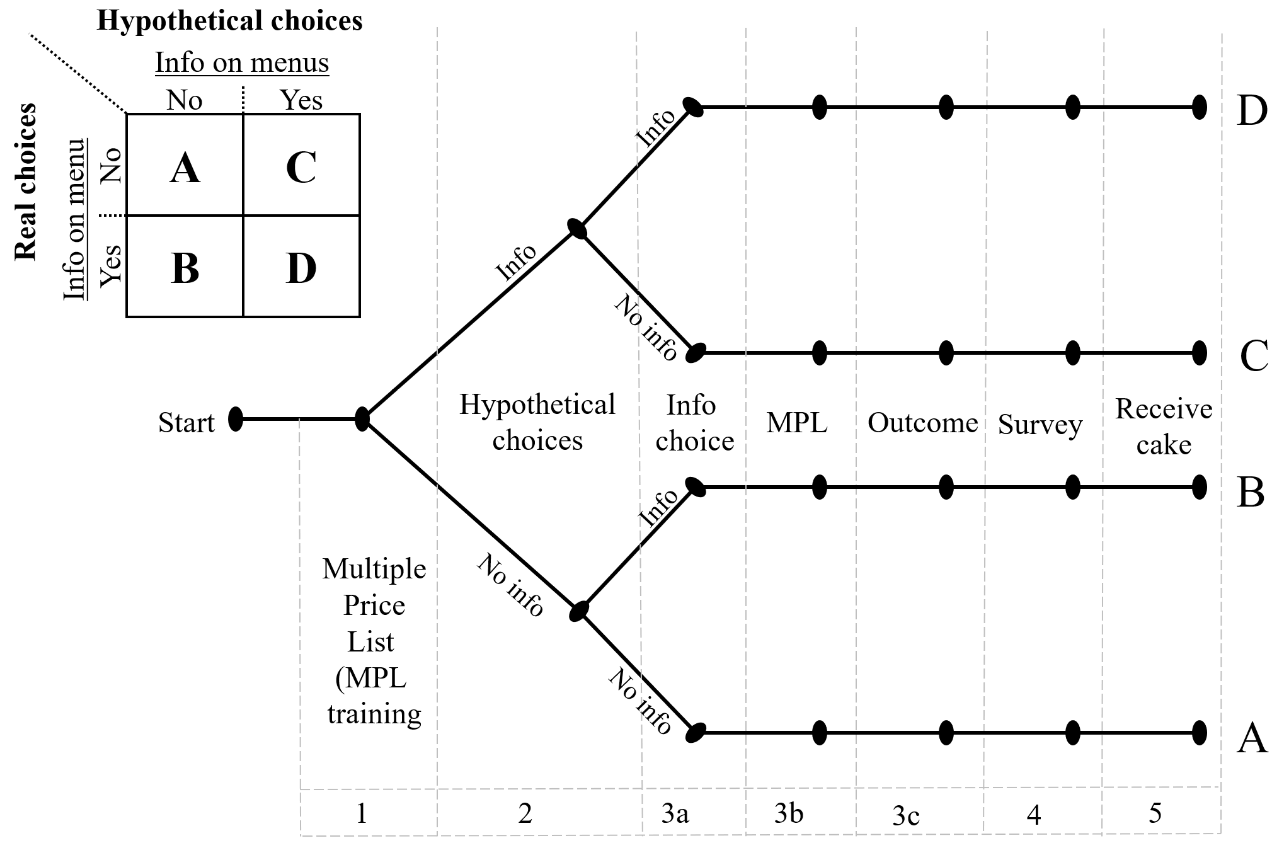
\includegraphics[width=1\textwidth]{./figures/experimentalDesign.png}}
  \end{center}
\end{figure}

Based on our recruitment flyer, all participants knew they would receive a cake for their participation in the experiment. After that, the experiment followed the structure shown in Figure \ref{fig:expDesign}. In step (1), we taught participants how to use a multiple-price list (MPL) and evaluated their understanding. In step (2), we asked participants to choose their preferred dessert from eleven consecutive dessert menus, each showing three desserts. These choices were not incentivized, and we were explicit about their hypothetical nature. In this step, we randomized half of the participants to see menus without calorie information and the other half to see menus with calorie information. The goal of this manipulation was to exercise some control over potential heterogeneity in expectations about information that participants might have brought to the laboratory. Making a series of choices from menus \emph{without} calorie information should set a baseline of \emph{low} expectations of receiving information when moving to the experiment’s next step, and making a series of choices from menus \emph{with} calorie information should set a baseline of \emph{high} expectations of receiving information.

In step (3a) participants were once again shown a menu with three new desserts. One of these, a cake, was marked as the dessert they were about to actually receive, to eat after the experiment.\footnote{We marked the cake they would receive for two reasons. First, we were not able to offer participants their dessert choice from a menu. As a compromise, to keep the menu structure used earlier, we marked the cake they would receive. Second, and more importantly, we wanted participants to focus on the choice of calorie information instead of the choice of dessert.} Within each baseline group established in step (2), we again randomized participants into two groups, resulting in a $2 \times 2$ design. One group was \emph{more endowed} with calorie information about the desserts, in the sense that the menu already showed a calorie-information column. However, the actual calorie numbers were \enquote{temporarily} \emph{xxx}-ed out, and participants in this group were asked whether they wanted to \enquote{keep} the calorie information, so they would see it, or \enquote{remove} the calorie information. The exact wording used is shown in Figure \ref{fig:expManipulation} (top panel). The other group was \emph{less endowed} with calorie information, in the sense that the menu showed nothing calorie-related to begin with. Participants in this group were asked whether they wanted to \enquote{add} calorie information, so they would see it, or \enquote{keep} calorie information \enquote{off}. The exact wording used is shown in Figure  \ref{fig:expManipulation} (bottom panel).

\begin{figure}[ht]
  \caption{Key experimental manipulation}\label{fig:expManipulation}
  \begin{center}
  {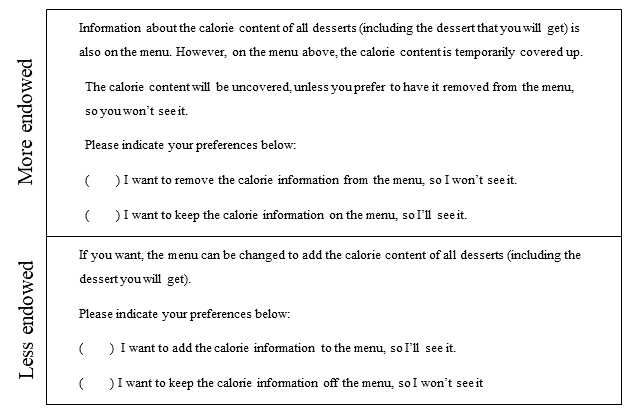
\includegraphics[width=1\textwidth]{./figures/keyManipulation.png}}
  \end{center}
\end{figure}

We argue that, compared to participants in the \emph{less endowed} treatment, participants in the \emph{more endowed} treatment were more likely to expect to receive calorie information about their cake, for three reasons. First, the presence of \emph{xxx}-ed out calorie-information column on the menu was intended to make \emph{more endowed} participants focus first on getting calorie information when considering whether they want to actually see it, whereas the absence of any such information for \emph{less endowed} participants was intended to make them focus first on not getting it. Second, the menu description pointed to the calorie information as already being on the menu for \emph{more endowed} participants, but as needing a change in the menu for \emph{less endowed} participants. And third, the description of how participants could choose to see the information used \enquote{I want to keep} for \emph{more endowed} participants, but \enquote{I want to add} for \emph{less endowed} participants.

% check usage of MPL

In step (3b) we aimed to elicit a monetary value for calorie information, using a multiple-price list that allowed this value to range from negative to positive. For example, if participants chose to see the calorie information in step (3a), thereby indicating that information had positive value for them, we gave them the option to either keep the information on the menu (i.e., stick with their initial choice and ultimately see the information) or remove the information and receive some additional money. That is, we elicited their Willingness To Accept (WTA) to \emph{not} see the information after all. Conversely, if participants chose not to see the information in step (3a), thereby indicating that information had negative value for them, we elicited their WTA to \emph{see} the information after all, in a similar fashion.

The multiple-price list included 10 choices, with monetary amounts ranging from \$0.01 to \$5.00.\footnote{The complete list of values in the MPL is \$0.01, \$0.25, \$0.50, \$0.75, \$1.00, \$1.50, \$2.00, \$2.50, \$3.00, and \$5.00.}  Once all 10 choices were made, one choice was randomly selected to be binding.

In step (3c), participants were shown a menu on which the calorie information of the cake they were about to receive was either revealed or not, depending on the outcome of the multiple-price list. In step (4), participants answered survey questions about their demographics, attitudes (risk preferences, time preferences, and degree of self-control), health status, health concern (the importance they assigned to their own health), and familiarity with calorie information (see Appendix \ref{appendix:background} for a description of these data). Finally, in step (5), participants received their payment (show-up fee plus earnings from the MPL) and cake.

\subsection{Identification strategy}

Based on our two consecutive manipulations to influence participants’ expectations about receiving calorie information, we organize participants in four groups: A, B, C, and D (see Figure \ref{fig:expDesign}). In the first manipulation, participants in groups A and B chose desserts from menus without calorie information, whereas participants in groups C and D chose desserts from menus with calorie information. In the second manipulation, participants in groups A and C chose whether to add information to a menu, whereas participants in groups B and D chose whether to keep information on a menu.

Because we are manipulating expectations, the timing and order of the manipulations matter. Specifically, for participants induced by the first manipulation to have high baseline expectations of receiving information (groups C and D), we expect the effect size of the second manipulation to be smaller. We therefore analyze that effect size separately for each baseline (i.e., groups A and B separately from groups C and D).

For each baseline, we identify the endowment effect by relating our experimental design to our theoretical definition of an endowment effect in equation \ref{eq:endowmentEffect}: $U(L^i|R^i)-U(L^u|R^i)>U(L^i|R^u)-U(L^u|R^u)$. For example, for participants induced by the first manipulation to have low baseline expectations of receiving information (groups A and B), being \emph{more endowed} with information in the second manipulation corresponds to having reference lottery $R^i$ (group B, left-hand side of the equation), while being \emph{less endowed} corresponds to having reference lottery $R^u$ (group A, right-hand side of the equation). Within each group, choosing to receive information corresponds to choosing outcome lottery $L^i$, while choosing not to receive information corresponds to choosing outcome lottery $R^u$. Thus, we can infer whether $U(L^i|R^i)-U(L^u|R^i)$ is positive ($L^i$ is chosen) or negative for each participant in group B, and similarly infer whether $U(L^i|R^u)-U(L^u|R^u)$ is positive or negative for each participant in group A. Then, we aggregate the choices of each group and simply compare the share of participants in group A who chose to receive information to the share of participants in group B who did so.\footnote{However, we note that our experimental results are contingent on the unverified manipulation of expectations (i.e., probabilistic beliefs). First, we assume that making eleven choices using menus with or without calorie information changes the probabilistic belief to expect to receive information. Second, given the probabilistic belief previously assumed to have been manipulated, we assume that presenting a menu with or without covered calorie information, along with other framing differences, would further change the probability belief to expect to receive information or not. We chose not to verify that the manipulations in fact had the intended effect in forming the expectation to receive information. One alternative would have been to ask participants whether they were expecting to receive information after each manipulation, however, we thought that such verification would have unintendedly changed the expectations. A second alternative would have been to use a different experimental design to manipulate the expectations. Following \citet{marzilliericsonExpectationsEndowmentsEvidence2011} \citet{heffetzEndowmentEffectExpectations2014}, one could manipulate the expectations, for example to expect to receive information, by telling participants that they have a 1\% chance to be able to choose whether to get the information or not, and a 99\% chance to receive the information (more recently, \citet{cerulli-harmsRandomizingEndowmentsExperimental2019} show that forced exchange is preferred than the allowable exchange used by \citet{marzilliericsonExpectationsEndowmentsEvidence2011} and \citet{heffetzEndowmentEffectExpectations2014}). The advantage of this approach is that one can verify that participants formed the correct expectations with a quiz evaluating the understanding of the statement. However, we think that our approach is more appropriate for the context of information and closer to potential policy applications outside of the laboratory. Overall, as reflected by the sensitivity of results to changes in the experimental environment documented in the empirical literature of expectations-based reference-dependent models, we can only conclude that manipulating expectations is a challenging task in which trade-offs are inevitable.} Furthermore, the heterogeneity in the data can be rationalized by assuming random utility.\footnote{Explicitly, participants could be heterogeneous (for example) in terms of self-control, curiosity, or concern about calorie intake.}

Our main goal is to show that preferences for information are not standard, and to propose that these preferences are reference-dependent. Therefore, we use the model of standard preferences as a straw man to set up null hypotheses to be rejected \citet{dellavignaChapterStructuralBehavioral2018}. Explicitly, we test the null hypothesis that the share of participants who choose to receive information is the same regardless of endowment status against the alternative that the share is higher for \emph{more endowed} participants. Note that the distinction between the DA approach and the KR approach does not play any role in the experiment: our design does not set out to distinguish between the two.\footnote{\citet{sprengerEndowmentEffectRisk2015} tests for the existence of an endowment effect for monetary risk using a design that does purposely distinguish between the DA and the KR approach. He shows that the data supports the KR approach instead of the DA approach.}

\subsection{Results}


We find evidence supporting the existence of an endowment effect for information: more participants chose to receive information when they were \emph{more endowed} with it (i.e., when getting a menu with temporarily \emph{xxx}-ed out calorie information). Furthermore, as expected, the effect was smaller for participants first primed to expect to receive information (i.e., participants who made initial hypothetical choices from menus with calorie information). A discussion of the empirical analysis and the results follows.

\subsubsection{Estimation strategy}

The practical goal of the analysis is to estimate the causal effect of receiving a menu with \emph{xxx}-ed out calorie information ($R^i$), relative to receiving a menu without \emph{xxx}-ed out calorie information ($R^u$), on the choice of receiving information ($L^i$) or not ($L^u$). Because we rely on the randomization process as identification strategy, unbiasedness of the unconditional ordinary least squares (OLS) estimator of the average treatment effect is guaranteed both under large- and finite-sample assumptions. However, the unbiasedness property guarantees only that the true treatment effect can be recovered by averaging the treatment effect over all potential realizations.\footnote{In general, the definition of a realization depends on the sources of uncertainty accounted for in the analysis. If only design-based uncertainty is considered, a realization is one draw of all possible randomizations within the population. If only sampling-based uncertainty is considered, a realization is one sample drawn from a superpopulation. Finally, if both sources of uncertainty are considered, a realization is a particular randomization from a particular sample \citep{abadieSamplingBasedDesignBasedUncertainty2020}.} In practice, however, we get only one estimate of the treatment effect, obtained from the one realization we observe. This observed estimate reflects, in addition to the true treatment effect, any imbalances between treatment groups of variables that are prognostic (i.e., correlated with the dependent variable). For example, if by chance one treatment group ends up with 70\% rather than 50\% of the female participants, and if being female is prognostic, then the estimate of the treatment effect will be influenced by the gender imbalance.

Given that our sample size for estimating the treatment effect of the key experimental manipulation is about 110 participants, the estimate is likely to reflect covariate imbalances. Consequently, to address the uncertainty regarding the extent to which these imbalances matter, we present estimates from both the unconditional OLS estimator and from all possible conditional OLS estimators that can be created by adjusting the regression with all combinations of the set of prognostic covariates with large imbalances between groups.\footnote{There are no objective criteria to define \emph{large}. The term is subjective and roughly means \enquote{large enough to affect the treatment effect in an economically significant way.} We describe the method used to identify the set of covariates with large imbalances between treatment groups in Appendix \ref{appendix:largeImbalances}.} Under large-sample assumptions, both the unconditional and the conditional estimators are unbiased. However, because the correlation between a covariate and the treatment variable might be different from zero, the conditional estimators present in our analyses are biased under finite-sample assumptions.\footnote{There are at least two alternatives to avoid the trade-off between unbiasedness and adjustments for covariate imbalance.

Ex-ante, one can use a randomized block design to force balance in prognostic covariates \citet{atheyChapterEconometricsRandomized2017}. However, this design requires a solid understanding of the covariates that are prognostic of information preferences, as well as baseline data with those prognostic covariates. For this study, it was not feasible to use a randomized block design, because we did not have the baseline data and we were not willing to compromise the incentivized choices in the experiment by asking survey questions up front.

Ex-post, if one can create binary covariates\textemdash from the original covariates\textemdash and they partition the population, the OLS estimator of the average treatment effect is unbiased when a full set of interactions is included \citep{linAgnosticNotesRegression2013,atheyChapterEconometricsRandomized2017}. This approach is not feasible for our study either because, even if we could create binary covariates that partition the population, we do not have enough observations to estimate the regression with a full set of interactions.
}

\subsubsection{Results using choice data}

We first present the results for participants not primed with calorie information (low baseline, groups A and B). The share of these participants who chose to receive information was $71\%$ for those \emph{more endowed} with information vs. $52\%$ for those \emph{less endowed} ($p=0.02$ from a $t$-test and $p=0.05$ from a Fisher’s exact test,  both one-sided).\footnote{We use Simon Heß’s Stata program ritest \citep{hessRandomizationInferenceStata2017} with 5000 random permutations and the coefficient of the treatment from an OLS regression as the test statistic for our Fisher’s exact tests \citet{imbensCausalInferenceStatistics2015}.} Figure \ref{fig:resultsLowBaseline} shows the implied treatment effect of $0.19$ and its associated $p$-value from an unconditional OLS regression, as well as 255 estimates and associated $p$-values from all possible adjusted regressions that can be estimated using the eight covariates with large imbalances between treatment groups A and B.

\begin{figure}[ht]
  \caption{Estimates of the treatment effect for participants in the \emph{low} baseline \\ (using choice data)}\label{fig:resultsLowBaseline}
  \begin{center}
  {\includegraphics[width=1\textwidth]{./figures/hypotheticalChoices_noInfo.png}}
  \end{center}
\end{figure}

Of these 256 point-estimates, 100\% are higher than $0.10$, 96.5\% are higher than $0.15$, and 20.1\% are higher than $0.20$. In addition, 99.6\%, 82\%, and 0\% of the estimates are statistically significant at the standard $0.1$, $0.05$, and $0.01$ levels of significance. Overall, we interpret these results as strong evidence for the existence of an endowment effect for information.

Next, we present the results for participants primed with calorie information (high baseline, groups C and D). The share of these participants who chose to receive information was 65.5\% for those \emph{more endowed} with information vs. 59.5\% for those \emph{less endowed} ($p=0.27$ from a $t$-test and $p=0.34$ from a Fisher’s exact test, both one-sided). Figure \ref{fig:resultsHighBaseline} shows the implied treatment effect of $0.06$ and its associated $p$-value from an unconditional OLS regression, as well as 512 estimates and associated $p$-values from all possible adjusted regressions that can be estimated using the nine covariates with large imbalances between treatment groups C and D.

\begin{figure}[ht]
  \caption{Estimates of the treatment effect for participants in the \emph{high} baseline \\ (using choice data)}\label{fig:resultsHighBaseline}
  \begin{center}
  {\includegraphics[width=1\textwidth]{./figures/hypotheticalChoices_info.png}}
  \end{center}
\end{figure}

Of these 512 point-estimates, 100\% are higher than $0$, 99.8\% are higher than $0.05$, 86\% are higher than $0.10$, 19\% are higher than $0.15$, and none are higher than $0.20$. In addition, 63\%, 10.5\%, and 0\% of the estimates are statistically significant at the standard $0.1$, $0.05$, and $0.01$ levels of significance. Overall, we interpret these results also as support for existence of an endowment effect\textemdash only one of the 512 point estimates is smaller than $0.05$. However, the size of the endowment effect is smaller for the primed participants of groups C and D than for the unprimed participants of groups A and B.

\subsubsection{Results using WTA data}

Finally, we designed the experiment to gather Willingness-To-Accept (WTA) data (from the multiple-price list) as an alternative measure of preferences for information. That is, we planned to reproduce the analyses presented above using, instead of the binary choice whether to receive information as a discrete dependent variable, WTA as a continuous dependent variable. Ex post, however, we realized that our way of eliciting WTA may not keep the relevant reference lottery constant, which makes it a questionable measure of participants’ value of information. For example, a participant randomized to receive a menu with \emph{xxx}-ed out calorie information (the \emph{more endowed} treatment) starts out with reference lottery $R^i$ and then chooses to either have the information revealed, corresponding to outcome lottery $L^i$, or taken off the menu, corresponding to outcome lottery $L^u$. From her choice, we obtain our binary measure of information preferences by inferring that $U(L^i|R^i)-U(L^u|R^i)$ is positive if $L^i$ is chosen, and negative if $L^u$ is chosen. If she chooses to receive information, we elicit her WTA to take the information off the menu after all. This WTA is plausibly a measure of the weakly positive utility $U(L^i|R^i)-U(L^u|R^i)$ that she forgoes by giving up information. If, however, she chooses to take the information off, we elicit her WTA to keep the information on after all, and have it be revealed. At that point, we lose control of her referent. Although the WTA measures the weakly positive utility $U(L^u|\cdot)-U(L^i|\cdot)$, it is unclear whether she still considers herself endowed with information, which would imply that her reference lottery when completing the multiple-price list is still $R^i$, or whether her initial choice to take the endowed information off the menu changes her reference lottery to $R^u$.

This lack of clarity reflects a broader gap in our understanding of the referent formation process. \citet{koszegiModelReferenceDependentPreferences2006} simply assume that the reference point depends on expectations held \enquote{in the recent past}, rather than expectations held at the time of consumption. They add that
\begin{displayquote}
  This does not assume that beliefs are slow to adjust to new information \emph{or that people are unaware of the choices that they have just made}\textemdash but that preferences do not instantaneously change when beliefs do. When somebody finds out five minutes ahead of time that she will for sure not receive a long-expected \$100, she would presumably immediately adjust her expectations to the new situation, but she will still five minutes later assess not getting the money as a loss. (p.1141, emphasis added).
\end{displayquote}

Applied to our context, this assumption implies that a participant’s choice of a particular outcome lottery need not instantaneously change her reference lottery. That is, she may still, at least for a while, feel endowed with information even if she just chose to give it up, or feel not endowed with information even if she just chose to get it.\footnote{Experimental results reported by \citet{heffetzAreReferencePoints2018} in fact suggest that reference points do not necessarily change to match beliefs even gradually, through the mere passage of time.  Instead, \enquote{some sense of internalization of, or getting used to, the new expectations} is required (p.5).}

Nevertheless, we cannot \emph{rule out} that a participant's choice to either receive or not receive information might have moved her referent before completing the multiple-price list. As a result, we cannot treat the difference in information values elicited through our multiple-price list for \emph{more endowed} and \emph{less endowed} participants as an estimate of the endowment effect expressed in dollar terms. What we can say is that, if an endowment effect does in fact exist, then any movement of participants' referents with their choices will bias downwards the elicited difference in information valuations.

The reason is straightforward. Let $\Re^i$ denote the subset of \emph{more endowed} participants, and $\Re^u$ the subset of \emph{less endowed} participants. If participants' choice did \emph{not} move their referents, then the endowment effect could be estimated as the average revealed value of information for \emph{more endowed} participants minus the average revealed value of information for \emph{less endowed} participants:
\begin{equation*}
  \frac{\sum_{j \in \Re^i}[U_j(L_j^i|R_j^i)-U_j(L_j^u|R_j^i)]}
       {|\Re^i|}
  -
  \frac{\sum_{j \in \Re^u}[U_j(L_j^i|R_j^u)-U_j(L_j^u|R_j^u)]}
      {|\Re^u|}.
\end{equation*}

If, on the other hand, participants' choices did move their referents, then the first average would be \enquote{contaminated} by some terms $U_j(L_j^i|R_j^u)-U_j(L_j^u|R_j^u)$, and the second average by some terms $U_j(L_j^i|R_j^i)-U_j(L_j^u|R_j^i)$. Suppose now that an endowment effect in fact exists (as defined in Equation \ref{eq:endowmentEffect}). Any contamination of the kind described will then tend to \emph{lower} the first average, since the contaminated terms $U_j(L_j^i|R_j^u)-U_j(L_j^u|R_j^u)$ will tend to be lower than the terms $U_j(L_j^i|R_j^i)-U_j(L_j^u|R_j^i)$ that they replace in the summation. Conversely, contamination will tend to \emph{raise} the second average, since the contaminated terms $U_j(L_j^i|R_j^i)-U_j(L_j^u|R_j^i)$ will tend to be higher than the terms $U_j(L_j^i|R_j^u)-U_j(L_j^u|R_j^u)$ that they replace. The upshot is that contamination will tend to reduce the estimated endowment effect relative to its true value.

Despite our potentially \emph{contaminated} estimates of the value of information, we still find that our results using WTA data are consistent with the existence of an endowment effect for information. We present the results for participants in the low and the high baseline below.\footnote{We follow \citet{allcottWelfareEffectsNudges2019} to calculate the value of the information for each participant from the choices in the multiple-price list. That is, we use the mean of the start and end points for the interior intervals and assume the conditional distribution of the WTA to be triangular for the open intervals. The results are robust to alternative assumptions (see the online supplementary material).}

For participants not primed with calorie information (low baseline, groups A and B), the average value of the information for those \emph{more endowed} was \$0.55 vs. \$0.08 for those \emph{less endowed} ($p=0.11$ from a $t$-test and $p=0.11$ from a Fisher's exact test, both one-sided). Figure \ref{fig:resultsLowBaselineWTA} shows the implied treatment effect of $0.46$ and its associated $p$-value from an unconditional OLS regression, as well as 256 estimates and associated $p$-values from all possible adjusted regressions that can be estimated using the eight covariates with large imbalances between groups A and B.

Of these 256 point-estimates, 100\% are higher than $\$0.2$, 94.15\% are higher than $\$0.25$, and 34.4\% are higher than $\$0.5$. In addition, 25.4\%, 6.64\%, and 0\%, of the estimates are statistically significant at the standard $0.1$, $0.05$, and $0.01$ levels of significance. Overall, we interpret also these results as support for the existence of the endowment effect\textemdash all 256 point-estimates are higher than $\$0.2$.

% ADD A NOTE OR FOOTNOTE ABOUT WHY RESULTS ARE WEAKER. CONTAMINATION AND LESS POWER TO DETECT EFFECT ARE TWO OF THEM. ????????????????????????????????

\begin{figure}[ht]
  \caption{Estimates of the treatment effect for participants in the \emph{low} baseline \\ (using WTA data)}\label{fig:resultsLowBaselineWTA}
  \begin{center}
  {\includegraphics[width=1\textwidth]{./figures/hypotheticalChoices_NoInfoWTA.png}}
  \end{center}
\end{figure}

For participants primed with calorie information (high baseline, groups C and D). The average value of the information for those \emph{more endowed} was \$0.56 vs. \$0.29 for those \emph{less endowed} ($p=0.24$ from a $t$-test and $p=0.21$ from a Fisher's exact test, both one-sided). Figure \ref{fig:resultsHighBaselineWTA} shows the implied treatment effect of $\$0.26$ and its associated $p$-value from an unconditional OLS regression, as well as 512 estimates and associated $p$-values from all possible adjusted regressions that can be estimated using the eight covariates with large imbalances between groups C and D.

Of these 512 point-estimates, 100\% are higher than $\$0.2$, 96.6\% are higher than $\$0.25$, and 0\% are higher than $\$0.5$. In addition, 15.6\%, 0\%, and 0\%, of the estimates are statistically significant at the standard $0.1$, $0.05$, and $0.01$ levels of significance. Overall, we interpret also these results as support for the existence of the endowment effect\textemdash all point-estimates are higher than $\$0.2$.

\begin{figure}[ht]
  \caption{Estimates of the treatment effect for participants in the \emph{high} baseline \\ (using WTA data)}\label{fig:resultsHighBaselineWTA}
  \begin{center}
  {\includegraphics[width=1\textwidth]{./figures/hypotheticalChoices_InfoWTA.png}}
  \end{center}
\end{figure}
